%%%%%%%%%%%%%%%%%%%%%%%%%%%%%%%%%%%%%%%%%
% Beamer Presentation
% LaTeX Template
% Version 1.0 (10/11/12)
%
% This template has been downloaded from:
% http://www.LaTeXTemplates.com
%
% License:
% CC BY-NC-SA 3.0 (http://creativecommons.org/licenses/by-nc-sa/3.0/)
%
%%%%%%%%%%%%%%%%%%%%%%%%%%%%%%%%%%%%%%%%%

%------------------------------------------------------------------------------------------------
% PACKAGES AND THEMES
%------------------------------------------------------------------------------------------------

\documentclass[table, xcolor = {dvipsnames}, 9pt]{beamer}
\usepackage{tikz}
\usetikzlibrary{calc}
\usetikzlibrary{positioning}
\usetikzlibrary{arrows.meta}
\usetikzlibrary{external}
\mode<presentation> {

% The Beamer class comes with a number of default slide themes
% which change the colors and layouts of slides. Below this is a list
% of all the themes, uncomment each in turn to see what they look like.

\usetheme{default}
%\usetheme{AnnArbor}
%\usetheme{Antibes}
%\usetheme{Bergen}
%\usetheme{Berkeley}
%\usetheme{Berlin}
%\usetheme{Boadilla}
%\usetheme{CambridgeUS}
%\usetheme{Copenhagen}
%\usetheme{Darmstadt}
%\usetheme{Dresden}
%\usetheme{Frankfurt}
%\usetheme{Goettingen}
%\usetheme{Hannover}
%\usetheme{Ilmenau}
%\usetheme{JuanLesPins}
%\usetheme{Luebeck}
%\usetheme{Madrid}
\usetheme{metropolis}
%\usetheme{Malmoe}
%\usetheme{Marburg}
%\usetheme{Montpellier}
%\usetheme{PaloAlto}
%\usetheme{Pittsburgh}
%\usetheme{Rochester}
%\usetheme{Singapore}
%\usetheme{Szeged}
%\usetheme{Warsaw}

% As well as themes, the Beamer class has a number of color themes
% for any slide theme. Uncomment each of these in turn to see how it
% changes the colors of your current slide theme.

%\usecolortheme{albatross}
%\usecolortheme{beaver}
%\usecolortheme{beetle}
%\usecolortheme{crane}
%\usecolortheme{dolphin}
%\usecolortheme{dove}
%\usecolortheme{fly}
%\usecolortheme{lily}
%\usecolortheme{orchid}
%\usecolortheme{rose}
\usecolortheme{seagull}
%\usecolortheme{seahorse}
%\usecolortheme{whale}
%\usecolortheme{wolverine}
\usefonttheme{professionalfonts}
%\setbeamertemplate{footline} % To remove the footer line in all slides uncomment this line
%\setbeamertemplate{footline}[page number] % To replace the footer line in all slides with a simple slide count uncomment this line

%\setbeamertemplate{navigation symbols}{} % To remove the navigation symbols from the bottom of all slides uncomment this line
}

\usepackage{graphicx} % Allows including images
\usepackage{booktabs} % Allows the use of \toprule, \midrule and \bottomrule in tables
\usepackage{tikz}
\usepackage{multirow}
\usepackage{natbib}
\usepackage{hyperref}
\usepackage{diagbox}
\usepackage{makecell}
\usepackage{xparse}
\usepackage{subfig}
\usepackage{amsmath}
\usepackage{amsfonts,amsthm,amsmath,amssymb}    
\usepackage{bbm}
\usepackage{bm}
\usepackage{empheq}
\usepackage{pgfplots}
\usepackage{animate}
\usepgfplotslibrary{colorbrewer}

\newcommand\mybox[2][]{\tikz[overlay]\node[fill=lightgray,inner sep=2pt, anchor=text, rectangle, rounded corners=1mm,#1] {#2};\phantom{#2}}
\hypersetup{unicode=true,
            bookmarksnumbered=true,
            bookmarksopen=true,
            bookmarksopenlevel=2,
            breaklinks=false,
            pdfborder={0 0 1},
            hypertexnames=false,
            pdfstartview={XYZ null null 1}}
\usepackage{xcolor}
\newcommand\myheading[1]{%
  \par\bigskip
  {\Large\bfseries#1}\par\smallskip}
\newcommand\given[1][]{\:#1\vert\:}
\theoremstyle{plain}
\newtheorem{thm}{Theorem}
\newtheorem{prop}{Proposition\thisthmnumber}
\newtheorem{lem}{Lemma\thisthmnumber}
\newtheorem{cor}{Corollary}
\newtheorem{defin}{Definition}
\newtheorem{algo}{Algorithm}
\newcommand*\diff{\mathop{}\!\mathrm{d}}
\newcommand*\Diff[1]{\mathop{}\!\mathrm{d^#1}}
\newcommand{\bh}[1]{{\color{blue}{#1}}}
\newcommand{\mh}[1]{{\color{magenta}{#1}}}
\newcommand{\thisthmnumber}{}
\newcommand{\tikzmark}[1]{\tikz[baseline,remember picture] \coordinate (#1) {};}
\newcommand*{\QEDA}{\hfill\ensuremath{\blacksquare}}%
\newcommand*{\QEDB}{\hfill\ensuremath{\square}}%
\DeclareMathOperator{\E}{\rm{E}}
\DeclareMathOperator{\R}{\mathbb{R}}
\DeclareMathOperator{\N}{\mathbb{N}}
\DeclareMathOperator{\Var}{\rm{Var}}
\DeclareMathOperator{\Cov}{\rm{Cov}}
\DeclareMathOperator{\Supp}{\rm{Supp}}
\DeclareMathOperator{\e}{\rm{e}}
\DeclareMathOperator{\F}{\mathcal{F}}
\DeclareMathOperator{\Z}{\mathcal{Z}}
\DeclareMathOperator{\logit}{\rm{logit}}
\DeclareMathOperator{\indep}{{\perp\!\!\!\perp}}
\DeclareMathOperator{\rank}{rank}
\DeclareMathOperator*{\argmin}{arg\,min}
\DeclareMathOperator*{\argmax}{arg\,max}
%\DeclareMathOperator{\Pr}{\rm{Pr}}
%------------------------------------------------------------------------
% TITLE PAGE
%-----------------------------------------------------------------------
\pagestyle{empty}
\title[]{Covariance adjustment in randomized experiments} % The short title appears at the bottom of every slide, the full title is only on the title page

\author{Thomas Leavitt} % Your name
\institute[] % Your institution as it will appear on the bottom of every slide, may be shorthand to save space
{
% Your institution for the title page
\medskip
\textit{} % Your email address
}
\date{\today} % Date, can be changed to a custom date

\begin{document}

\begin{frame}
\titlepage % Print the title page as the first slide
\end{frame}

%\begin{frame}
%\frametitle{Overview} % Table of contents slide, comment this block out to remove it
%\tableofcontents % Throughout your presentation, if you choose to use \section{} and \subsection{} commands, these will automatically be printed on this slide as an overview of your presentation
%\end{frame}

%------------------------------------------------------------------------
% PRESENTATION SLIDES
%------------------------------------------------------------------------
\begin{frame}{Covariance adjustment in randomized experiments}
\vfill
\begin{itemize}
\item We often have information contained in baseline covariates \vfill
\begin{itemize} \vfill
\item I.e., variables measured \textbf{before} treatment assignment  \vfill
\end{itemize} \vfill
\item If baseline covariates related to POs, we want to use covariates to increase\vfill
\begin{enumerate}
\item Precision of estimators \vfill 
\item Power of tests \vfill
\end{enumerate} \vfill
\end{itemize} \vfill
\end{frame}
%------------------------------------------------------------------------
\begin{frame}{Covariance adjustment in randomized experiments}
\vfill
\begin{itemize}
\item Two primary approaches to covariate adjustment  \vfill
\begin{enumerate} \vfill
\item Random assignment within blocks of units similar in covariates  \vfill
\item Rescaling outcome to make its variance smaller  \vfill
\end{enumerate}  \vfill
\end{itemize} \vfill
\end{frame}
%------------------------------------------------------------------------
\section{Block random assignment}
\begin{frame}{Block random assignment}
\vfill
\begin{itemize} \vfill
\item Construct blocks of units similar in baseline covariates related to POs \vfill
\item By blocking we reduce number of possible assignments \vfill
\begin{itemize} \vfill
\item Goal is to exclude assignments yielding estimates far from truth \\ so that estimator will be closer to truth, on average \vfill
\end{itemize} \vfill
\end{itemize} \vfill
\end{frame}
%------------------------------------------------------------------------
\begin{frame}{Block random assignment: Example}
\vfill
\textcolor{magenta}{Example}: Experiment with $N = 6$ units, $n_1 = 3$ and $n_0= 3$
\begin{table}[H]
\centering
\begin{tabular}{l|l|l|l}
$\bm{y}(\bm{0})$ & $\bm{y}(\bm{0})$ & $\bm{\tau}$ & $\bm{x}$ \\ \hline
  20 & 22 & 2 & 1 \\
  8 & 12 & 4 & 1 \\
  11 & 11 & 0 & 0 \\
  10 & 15 & 5 & 1 \\
  14 & 18 & 4 & 1 \\
  1 &  4 & 3 & 0 \\
    \end{tabular}
\caption{True values of $\bm{y}(\bm{0})$, $\bm{y}(\bm{0})$, $\bm{\tau}$ and baseline covariate $\bm{x}$}
\end{table} \vfill
Stratify on $\bm{x}$ and assign half of units to treatment within strata \vfill

In this case, instead of $\binom{6}{3} = 20$ assignments, we have $\prod \limits_{b = 1}^B \binom{N_b}{n_{1,b}} = 12$ assignments, where $b = 1, \ldots , B$ indexes the blocks \vfill
\end{frame}
%------------------------------------------------------------------------
\begin{frame}{Block random assignment: Example}
\vfill
\begin{itemize} \vfill
\item Set of assignments under block random assignment \vfill
\item Units with \mh{$x_i = 1$}; units with \bh{$x_i = 0$} \vfill
\end{itemize} 
\vfill
\begin{equation*}
\Omega =
\left\{
\begin{bmatrix} \mh{1} \\ \mh{1} \\ \bh{1} \\ \mh{0} \\ \mh{0} \\ \bh{0} \end{bmatrix},
\begin{bmatrix} \mh{1} \\ \mh{1} \\ \bh{0} \\ \mh{0} \\ \mh{0} \\ \bh{1} \end{bmatrix},
\begin{bmatrix} \mh{1} \\ \mh{0} \\ \bh{1} \\ \mh{1} \\ \mh{0} \\ \bh{0} \end{bmatrix},
\begin{bmatrix} \mh{1} \\ \mh{0} \\ \bh{1} \\ \mh{0} \\ \mh{1} \\ \bh{0} \end{bmatrix},
\begin{bmatrix} \mh{1} \\ \mh{0} \\ \bh{0} \\ \mh{1} \\ \mh{0} \\ \bh{1} \end{bmatrix},
\begin{bmatrix} \mh{1} \\ \mh{0} \\ \bh{0} \\ \mh{0} \\ \mh{1} \\ \bh{1} \end{bmatrix},
\begin{bmatrix} \mh{0} \\ \mh{1} \\ \bh{1} \\ \mh{1} \\ \mh{0} \\ \bh{0} \end{bmatrix},
\begin{bmatrix} \mh{0} \\ \mh{1} \\ \bh{1} \\ \mh{0} \\ \mh{1} \\ \bh{0} \end{bmatrix},
\begin{bmatrix} \mh{0} \\ \mh{1} \\ \bh{0} \\ \mh{1} \\ \mh{0} \\ \bh{1} \end{bmatrix},
\begin{bmatrix} \mh{0} \\ \mh{1} \\ \bh{0} \\ \mh{0} \\ \mh{1} \\ \bh{1} \end{bmatrix},
\begin{bmatrix} \mh{0} \\ \mh{0} \\ \bh{1} \\ \mh{1} \\ \mh{1} \\ \bh{0} \end{bmatrix},
\begin{bmatrix} \mh{0} \\ \mh{0} \\ \bh{0} \\ \mh{1} \\ \mh{1} \\ \bh{1} \end{bmatrix}
\right\}.
\label{eq: example block omega}
\end{equation*}
\vfill
\begin{itemize}
\item Only $12$ assignments (instead of 20) because half of units w/ $\mh{x_i = 1}$ treated and half of units w/ $\bh{x_i = 0}$ treated
\end{itemize}
\end{frame}%------------------------------------------------------------------------
\begin{frame}{Block random assignment: Example}
\begin{figure}[H]
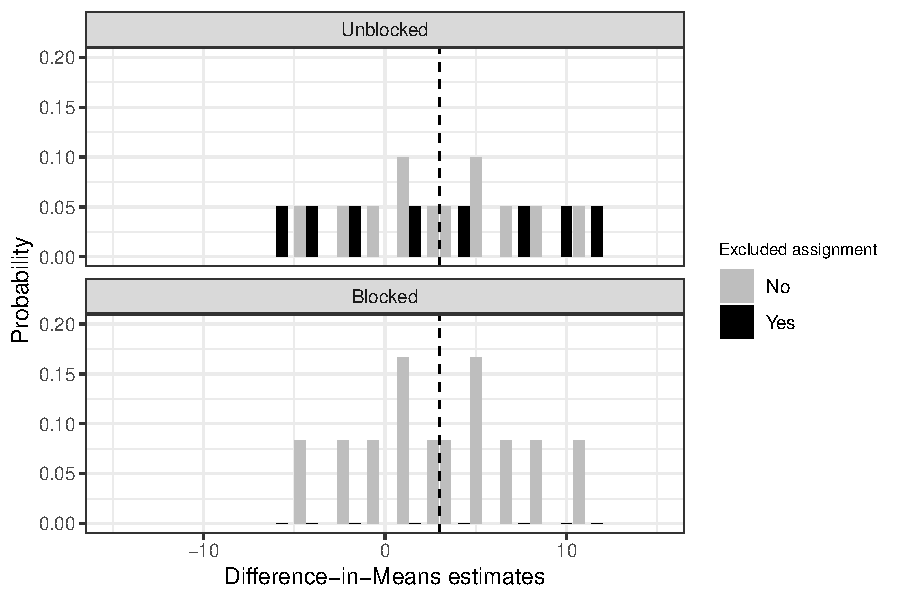
\includegraphics[width = \linewidth]{blocked_assign_plot.pdf}
\caption{Difference-in-Means distribution under unblocked and blocked assignment}
\end{figure}
\end{frame}%------------------------------------------------------------------------
\section{Rescaling outcomes}
\begin{frame}{Rescaling outcomes}
\vfill
\begin{itemize} \vfill
\item Variance of Diff-in-Means \vfill
\begin{equation*}
\Var\left[\hat{\tau}\left(\bm{Z}, \bm{Y}\right)\right] = \frac{1}{N - 1}\left(\frac{n_1 \mh{\sigma^2_{\bm{y}(\bm{0})}}}{n_0} + \frac{n_0\mh{\sigma^2_{\bm{y}(\bm{1})}}}{n_1} + 2\mh{\sigma_{\bm{y}(\bm{0}), \bm{y}(\bm{1})}}\right)
\end{equation*} \vfill
\item Can we rescale outcomes so that $\mh{\sigma^2_{\bm{y}(\bm{0})}}$ and $\mh{\sigma^2_{\bm{y}(\bm{1})}}$ are smaller?  \vfill
\item[$\star$] Residualizing cannot alter individual treatment effects
\begin{align*}
y_{i}(1) - f(\bm{x}_i) - \left[y_{i}(0) - f(\bm{x}_i)\right] & = y_{i}(1) - f(\bm{x}_i) - y_{i}(0) + f(\bm{x}_i) \\ 
& = y_{i}(1) - y_{i}(0) \\ 
& = \tau_i,
\end{align*}\vfill
where $f(\cdot)$ is function that predicts outcome from $\bm{x}_i \in \R^K$ \\ 
\citep{rosenbaum2002c} \vfill
\item Ideally, $f(\cdot)$ fit to historical data or set-aside sample not in experiment \vfill
\end{itemize} \vfill
\end{frame}
%------------------------------------------------------------------------
\begin{frame}{Rescaling outcomes}
\vfill
\begin{itemize} \vfill
\item \textcolor{magenta}{Example}: Acorn GOTV experiment \citep{arceneaux2005}
\end{itemize} 
\begin{center}
  \begin{tabular}{r|rrr}
  \hline
 & GOTV? & vote03 (\%) & vote03 - vote02 (\%) \\
  \hline
1 & 0 & 38 & -36 \\
$\vdots$& $\vdots$& $\vdots$ & $\vdots$ \\
13 & 0 & 19 & -38 \\
14 & 0 & 34 & -27 \\
15 & 1 & 49 & -25 \\
16 & 1 & 38 & -28 \\
$\vdots$& $\vdots$& $\vdots$ & \\
28 & 1 & 29 & -32\\
   \hline
\end{tabular}
\end{center} \vfill
Conduct analysis on rescaled vote03 - vote02 (\%) outcome
\end{frame}
%-------------------------------------------------------------------------------------
\begin{frame}{Rescaling outcomes} \vfill
\begin{figure}[H]
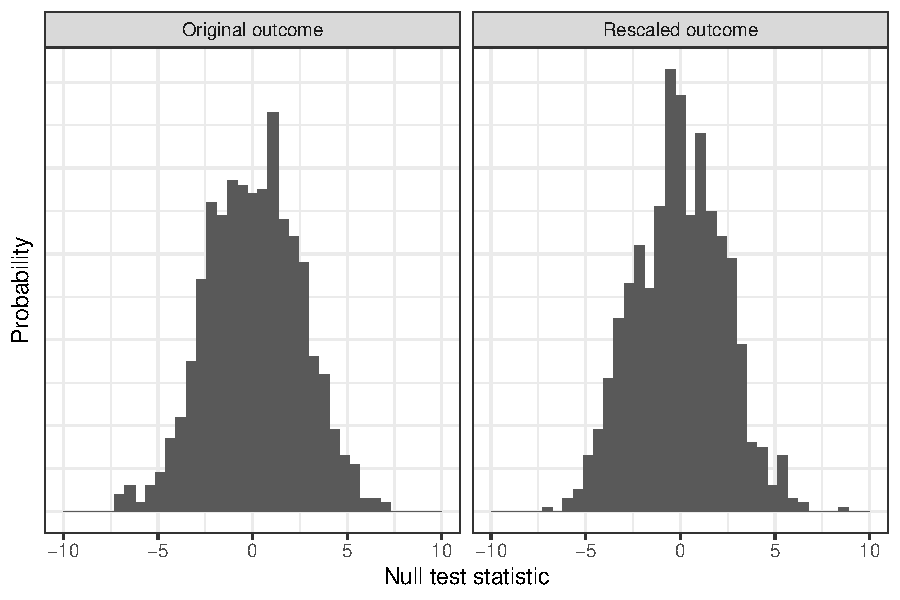
\includegraphics[width = \linewidth]{null_dist_no_effect_plot.pdf}
\caption{Difference-in-Means under sharp null on original and rescaled outcomes}
\end{figure}
\end{frame}
%-------------------------------------------------------------------------------------
\section{Regression Adjustment}
\begin{frame}{Linear regression} \vfill
\begin{itemize} \vfill
\item Common tool for incorporating info from covariates \vfill
\item Usual regression assumptions \vfill
\begin{itemize} \vfill
\item Independent and identically distributed observations \vfill
\item Outcome conditional on predictors, $Y \given X$, is Normally distributed \vfill
\end{itemize} \vfill
\item In our setting, \vfill
\begin{itemize}
\item Potential outcomes fixed (non-random) quantities \vfill
\item Experimental subjects \textbf{not} sampled from superpopulation \vfill
\item Randomness due only to assignment process \vfill
\end{itemize}  
\item \textcolor{magenta}{Is regression w/out standard assumptions still useful?}
\end{itemize} \vfill
\end{frame}
%-------------------------------------------------------------------------------------
\begin{frame}{Regression: No covariate adjustment} \vfill
\begin{itemize} \vfill
\item Suppose only SUTVA and complete random assignment \\ (not the usual regression assumptions) \vfill
\begin{itemize} \vfill
\item W/out covariate adjustment, $\bm{z}$'s estimated coeff equivalent to Diff-in-Means \vfill
\item[] \texttt{coef(lm(formula = y $\sim$ z, data = data))["z"]} \vfill
\item HC2 standard error equivalent to Neyman's conservative variance estimator \vfill
\item[] \texttt{library(sandwich)} \\ 
\item[] \texttt{diag(vcovHC(x = mod, type = "HC2"))["z"]}
\end{itemize} \vfill
\item \textcolor{magenta}{How does regression perform with covariate adjustment?} \\ \citep{freedman2008a,freedman2008b,lin2013,cohenfogarty2023} \vfill
\end{itemize} \vfill
\end{frame}
%-------------------------------------------------------------------------------------
\begin{frame}{Regression: With covariate adjustment} \vfill
\begin{figure}[H]
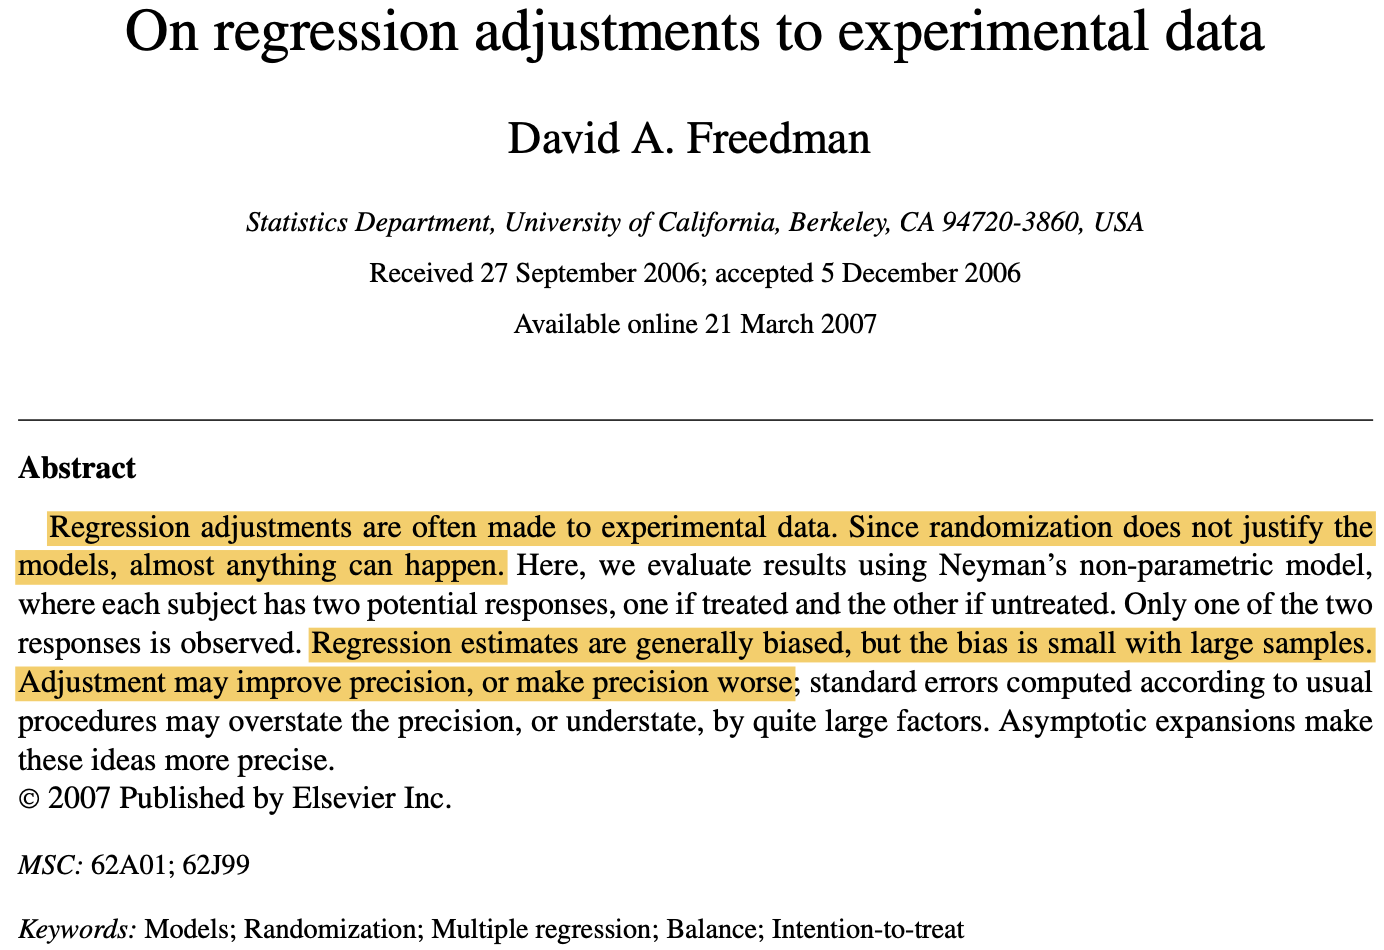
\includegraphics[width=0.9\linewidth]{Freedman_2008.png}
\caption{Freedman (2008), p.~180}
\end{figure}
\end{frame}
%------------------------------------------------------------------------
\begin{frame}{Regression} \vfill
\begin{figure}[H]
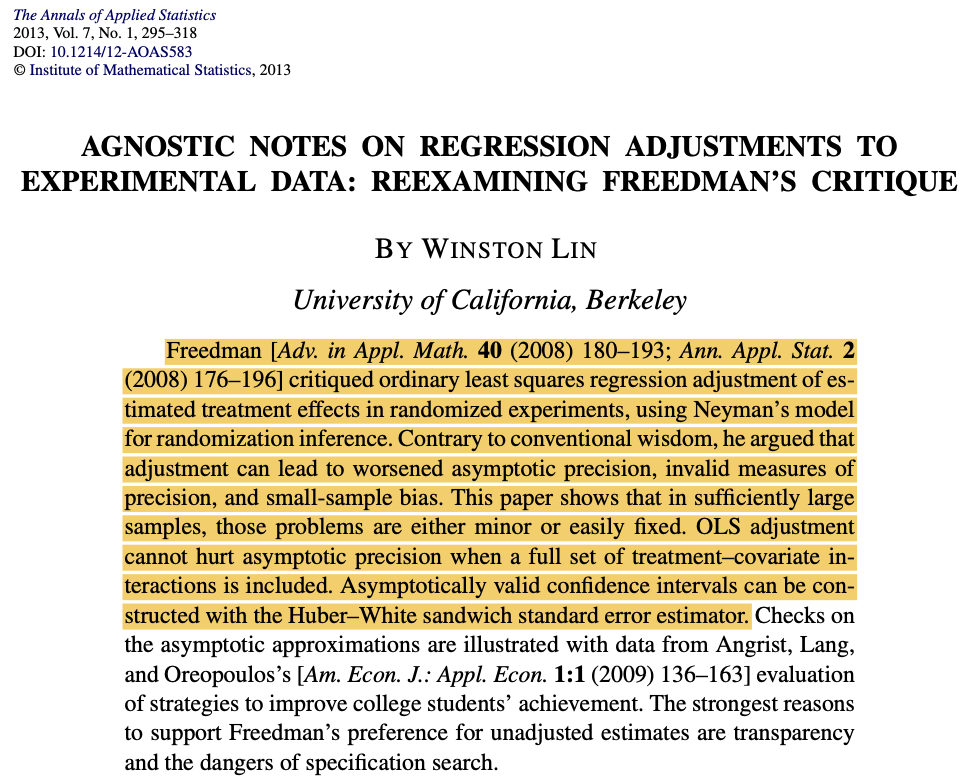
\includegraphics[width=0.9\linewidth]{Lin_2013.png}
\caption{Lin (2013), p.~295}
\end{figure}
\end{frame}
%------------------------------------------------------------------------
\begin{frame}{Linear regression} \vfill
\begin{itemize} \vfill
\item \citet{lin2013} shows regression w/ full set of treatment-covariate interactions \vfill
\begin{itemize} \vfill
\item Consistent for average treatment effect \\ (but may have bias in small experiments) \vfill
\item Robust HC2 variance estimator satisfies ``do-no-harm'' property \vfill
\begin{itemize} \vfill
\item W/ large $N$, regression cannot make variance larger than Diff-in-Means' variance \\ (Usually regression will decrease variance) \vfill
\end{itemize} \vfill
\end{itemize} \vfill
\item To implement Lin estimator in \texttt{R} \vfill
\item[] \texttt{library(estimatr)}
\item[]\texttt{lm\_lin(y $\sim$ z, covariates = x\_1 + x\_2, data = data)} \vfill 
\item Equivalent to
\item[] \texttt{lm(formula = y $\sim$ z + x\_1\_cent + x\_2\_cent + z * x\_1\_cent + z * x\_2\_cent, data = data)}
\end{itemize}  
\end{frame}
%------------------------------------------------------------------------
\begin{frame}{Nonlinear regression} \vfill
\begin{itemize}
\item ``The logit model is often used to analyze experimental data. However, randomization does not justify the model'' \citep[][p.~237]{freedman2008b}. \vfill
\item Argument analogous to \citet{lin2013} applies for nonlinear covariate adjustment \vfill
\begin{itemize} \vfill
\item E.g., logistic regression, Poisson regression, etc. \vfill
\end{itemize} \vfill
\item See \citet{cohenfogarty2023} for details \vfill
\end{itemize}  \vfill
\end{frame}
%------------------------------------------------------------------------
\begin{frame}[allowframebreaks]
\frametitle{References} 
\scriptsize
\bibliographystyle{chicago}
\bibliography{Bibliography.bib}   % name your BibTeX data base
\end{frame}
%-------------------------------------------------------------------------------------
\end{document}